\section{Deep Linearly Gated Networks: Complete Disentanglement}
{\centering $\text{DLGN} : x\rightarrow \stackrel{\text{Primal} }{\text{Linear}}\rightarrow \text{Pre-activations}\rightarrow\text{Gates}\stackrel{\text{lifting}}{\rightarrow} \phi_{\Tf}(x) {\rightarrow}\stackrel{\text{Dual} }{\text{Linear}}: \hat{y}(x)=\ip{\phi_{\Tf}(x),v_{\Tv}}$ \par}
 %We continue to be in the DGN setting of characterising learning the weights with fixed gates in the limit of infinite width as in \Cref{sec:fixedgates}. We already saw that this setting is characterised by the NPK. 
%In this section is to present new theoretical insights on prior result and new theoretical results with insights to justify the claim that the learning of the weights given the gates is \emph{disentangled in the path space}. By this, we mean that it is enough to think that the value network is dual linear, i.e., it simply computes/learns the inner product $\hat{y}_{\text{DGN}}=\ip{\phi_{\Tf}(x),v_{\Tv}}$. There are two compelling reasons to adopt the dual view. Reason-(i): In \Cref{sec:gatelearning} we saw that the fixed learnt gates ($79.68\%$) recover almost all the performance of the DNN ($80.32\%$), i.e., dual linearity is not a mere conceptualisation, but is analogous to a linear model in practice as well. In other words, just like one can learn weight vector in a linear model given the features, one can learn the neural path value given the neural path features. Reason-(ii): in the fixed gates infinite width setting, we  already have an interpretation via the NPK.

%In this section is to present new theoretical insights and results to justify the claim that value network is \emph{disentangled in the path space}. By this, we mean that it is enough to think that the value network computes/learns the inner product $\hat{y}_{\text{DGN}}=\ip{\phi_{\Tf}(x),v_{\Tv}}$. There are two compelling reasons to adopt the dual view. Reason-(i): In \Cref{sec:gatelearning} we saw that the fixed learnt gates ($\mathbf{79.68\%}$) recover almost all the performance of the DNN ($\mathbf{80.32\%}$), i.e., dual linearity is not a mere conceptualisation, but is analogous to a linear model in practice as well. In other words, just like one can learn weight vector in a linear model given the features, one can learn the neural path value given the neural path features. Reason-(ii): in the fixed gates infinite width setting, we have an interpretation via the NPK.

The deep linear gated network (DLGN) has two `mathematically' interpretable linearities, the `primal' and the `dual' linearities. The primal linearity is ensured in via construction and needs no theoretical justification. Once the pre-activations triggers gates, $\phi_{\Tf}(x)$ gets realised in the value network by activating the paths.  Now, the value network itself is `dual' linear, i.e., it simply computes/learns the inner product $\hat{y}(x)=\ip{\phi_{\Tf}(x),v_{\Tv}}$. Gating \emph{lifts} the `primal' linear computations in the feature network to `dual' linear computations in the value network. Dual linearity is characterised by the NPK (for infinite width) which in turn depends on the input and gates, and  the fact that the pre-activations to the gates are primal linear implies complete disentanglement and interpretability. 

Dual linearity, while being mathematically evident due to the inner product relationship, adopting it has the following conceptual issue: it is a commonly held view that `sophisticated features are learnt in the layers', that is, given that the input $x\in\R^{\din}$  is presented to the value network (as in \Cref{fig:dgn}), it could be argued that the GaLUs and linear operations are entangled which in turn enable learning of sophisticated features in the layers. In what follows, we demystify this layer-by-layer view via theory (infinite width case) in \Cref{sec:analysis} , and experiments (on finite width networks) in \Cref{sec:dlgn}, and then study the performance of DLGN in \Cref{sec:dlgn}. The layer-by-layer view is demystified by showing that (i) a constant $\mathbf{1}$ input can be given to the value network, (ii) layer-by-layer can be destroyed. The constant $\mathbf{1}$ input is meant to show that if the input is not given to the value network then it is not possible to learn sophisticated structures `from the input' in a layer-by-layer manner.  In terms of the dual linearity, providing a constant $\mathbf{1}$ input has only a minor impact, in that, the neural path feature becomes $\phi(x,p)=1\cdot A(x,p)$, i.e., it still encodes the path activity which is still input dependent. Since $\phi(x)$ depends only on gates, the NPK will depend only on the $\textbf{overlap}$ matrix; results in \Cref{sec:analysis}  captures this in theory. Now, it could be argued that, despite a constant $\mathbf{1}$ input, the gates are still arranged layer-by-layer, due to which, the value network is still able to learn sophisticated structures in its layers. \Cref{sec:analysis} has theory that points out that as long as the \textbf{correlation of the gates} is not lost, the layer-by-layer structure can be destroyed.
% 
%The conceptual issue that stops us from adopting the dual view is the commonly held view that `sophisticated features are learnt in a layer-by-layer' manner. That is, in a DGN, given that the input $x\in\R^{\din}$  is presented to the value network, it could be argued that the GaLUs and linear operations are entangled which in turn enable learning of sophisticated features in the layers. To demystify the layer-by-layer processing viewpoint, in the DGN and DLGN the value network can be provided with a constant $\mathbf{1}$. This is to show that if the input $x\in\R^{\din}$ is not given to the value network in the first place it is not possible to learn sophisticated structures in a layer-by-layer manner. In terms of the dual linearity, providing a constant $\mathbf{1}$ input has only a minor impact, in that, the neural path feature becomes $\phi(x,p)=1\cdot A(x,p)$, i.e., it still encodes the path activity which is still input dependent. Since $\phi(x)$ depends only on gates, the NPK will depend only on the $\textbf{overlap}$ matrix; all the theoretical results in this section will capture the effect. Now, it could be argued that, despite a constant $\mathbf{1}$ input, the gates are still arranged layer-by-layer, due to which, the network is able to still learn sophisticated structures in a layer-by-layer manner. All the results in this section will point out that as long as the \textbf{correlation of the gates} is not lost, the layer-by-layer structure can be destroyed.
\subsection{Dual Linearity: New Insights and New Results}\label{sec:analysis}
%We saw in \Cref{sec:fixedgates} that dual linearity is characterised by the NPK for infinite width case. We now present new insights on \Cref{th:fcprev} by restating it explicitly in terms of the gates in \Cref{th:fc}. We present new results to reveal additional structure of the NPK in the presence of convolutions with global-average-pooling and skip connections in \Cref{th:conv,th:res} respectively and discuss how structure of the NPK helps in demystifying the layer-by-layer view. The motivation for \Cref{th:conv,th:res} that convolutions with pooling and skip connections are quite standard architectural choices and the disentanglement should handle these as well.
%We saw in \Cref{sec:fixedgates} that dual linearity is characterised by the NPK for infinite width case. We now present new insights on \Cref{th:fcprev} by restating it explicitly in terms of the gates in \Cref{th:fc}. Prior work on dual view was for fully connected networks. In this paper, we present new results to reveal additional structure of the NPK in the presence of standard architectural choices namely convolutions with global-average-pooling and skip connections in \Cref{th:conv,th:res} respectively and discuss how structure of the NPK helps in demystifying the layer-by-layer view.
%We saw in \Cref{sec:fixedgates} that dual linearity is characterised by the NPK for infinite width case. We now present new insights on \Cref{th:fcprev} by restating it explicitly in terms of the gates in \Cref{th:fc}. We present new results to reveal additional structure of the NPK in the presence of standard architectural choices namely convolutions with global-average-pooling and skip connections in \Cref{th:conv,th:res} respectively and discuss how  NPK structure helps in demystifying the layer-by-layer view.
We saw in \Cref{sec:fixedgates} that dual linearity is characterised by the NPK for infinite width case. In this section, we: (i) cover standard architectural choices namely convolutions with global-average-pooling and skip connections in \Cref{th:conv,th:res}; the prior result \Cref{th:fcprev} is only for the fully connected case, (ii)  present new insights on \Cref{th:fcprev} by restating it explicitly in terms of the gates in \Cref{th:fc}, and (iii) discuss how the NPK structure helps in demystifying the layer-by-layer view. Note: Results in this section are about the value network and hold for both DGN and DLGN.
%In what follows, we first restate the prior result. While \Cref{th:fc} and Theorem 5.1 in \citep{npk} are mathematically identical, \Cref{th:fc} is written in a manner to capture the fact that the NPK is invariant to permutation of the layers. \Cref{th:conv,th:res} are entirely new and are extensions of the dual view for convolutions with global pooling and skip connections. 


%\subsection{NPK of FC-DNN: Product Kernel }
%\input{cnpkexample}
%\subsection{Neural Path Kernel : Similarity based on active sub-networks}
%\textbf{Remark.} In the case of fully connected networks, $\textbf{overlap}_{\Theta}(i,x,x')$ is equal for all $i\in[\din]$, and hence $\text{NPK}_{\Theta}(x,x')=\ip{x,x'}\cdot\textbf{overlap}_{\Theta}(x,x')$.
%We point out that this statistical decoupling of weights and gates in \Cref{assmp:main} is unrealisable in a DNN with ReLU, however, this assumption can be trivially realised in a DGN. %Further, we are interested only in the `what?' ( and not `how?') question related to the gates in which case this assumptions is not a restriction.
\subsubsection{Fully Connected: Product of LayerWise Base Kernels}
\begin{theorem}
\label{th:fc} Let $G_l(x)\in[0,1]^w$ denote the gates in layer $l\in\{1,\ldots,d-1\}$ for input $x\in\R^{\din}$. Under \Cref{assmp:main}  ($\sigma=\frac{\cscale}{\sqrt{w}}$) as $w\rightarrow \infty $, we have for fully connected DGN/DLGN:
\begin{align*}
\text{NTK}^{\texttt{FC}}(x,x') \rightarrow d \cdot \sigma^{2(d-1)} \cdot \text{NPK}^{\texttt{FC}}(x,x') = d \cdot \cscale^{2(d-1)} \cdot \left(\ip{ x,x'} \cdot \Pi_{l=1}^{d-1} \frac{\ip{G_l(x),G_l(x')}}w\right),
\end{align*}
\end{theorem} 
$\bullet$ \textbf{Product Kernel : Role of Depth and Width.} \Cref{th:fc} is mathematically equivalent to  \Cref{th:fcprev}, which follows from the observation that $\textbf{overlap}(x,x')=\Pi_{l=1}^{(d-1)}\ip{G_l(x),G_l(x')}$. While this observation is very elementary in itself, it is significant at the same time;  \Cref{th:fc} provides the most simplest kernel expression that characterises the information in the gates. From \Cref{th:fc} it is evident that the role of width is \emph{averaging} (due to the division by $w$). Each layer therefore corresponds to a \emph{base kernel} $\frac{\ip{G_l(x),G_l(x')}}w$ which measures the \emph{\textbf{correlation of the gates}}. The role of depth is to provide the product of kernels. To elaborate, the feature network provides the gates $G_l(x)$, and the value network realises the product kernel in \Cref{th:fc} by laying out the GaLUs depth-wise, and connecting them to form a deep network. The depth-wise layout is important: for instance, if we were to concatenate the gating features as $\varphi(x)=(G_l(x),l=1,\ldots,d-1)\in\{0,1\}^{(d-1)w}$, it would have only resulted in the kernel $\ip{\varphi(x),\varphi(x')}=\sum_{l=1}^{d-1}{\ip{G_l(x),G_l(x')}}$, i.e., a \emph{sum  (not product)} of kernels. 

$\bullet$ \textbf{Constant $\mathbf{1}$ Input.} This has a minor impact, in that, the expression on right hand side of \Cref{th:fc} becomes $d \cdot \cscale^{2(d-1)} \cdot \din \cdot \Pi_{l=1}^{d-1} \frac{\ip{G_l(x),G_l(x')}}w$, i.e., the kernel still has information of the gates.

$\bullet$ \textbf{Destroying structure by permuting the layers.}  $\Pi_{l=1}^{d-1} \frac{\ip{G_l(x),G_l(x')}}w$ is permutation invariant, and hence permuting the layers has no effect.


%\textbf{Remark.} Here $\frac{\ip{G_l(x),G_l(x')}}w$ are the \emph{base kernels} measuring the \emph{\textbf{correlation of the gates}}. We show experimentally that the correlation of gates is essentially  `what is learnt in a DNN with ReLUs'.
%and $\Pi_{l=1}^{d-1} \frac{\ip{G_l(x),G_l(x')}}w$ is a product of these base kernels and hence the name `Product of Kernels Theorem'.  The base kernels are essentially measuring which we show via  We now list the roles of the two networks, weights, depth and width.

%\textbf{Feature Network.} The role of this network is to process the input layer-by-layer and produce the $w$-dimensional gating features $G_l(\cdot)$. Each layer comprises of `$w$' ReLUs, and a given ReLU (i.e., gate) is `on' if the input to that layer lies on the positive half-space of hyperplane of given by the incoming weights of that ReLU. Thus the gates of a given layer are based on the angle between the input to that layer and the various hyperplanes given by the weights of that layer. Prior experiments in [\citenum{npk}] and the experiments in this paper show that the feature network, i.e., the gates hold most information, which in turn means that weights of the feature network are key.

%\textbf{Value Network}. The value network implements the product of kernels by laying out the gates as masks depth-wise, and connecting them in the structure of a DNN. Note that depth-wise layout plays an important role here: for instance, if we were to concatenate the gating features as $\varphi(x)=(G_l(x),l=1,\ldots,d-1)\in\{0,1\}^{(d-1)w}$, it would have only resulted in the kernel $\ip{\varphi(x),\varphi(x')}=\sum_{l=1}^{d-1}{\ip{G_l(x),G_l(x')}}$, i.e., a \emph{sum  (not product)} of kernels. Prior experiments in [\citenum{npk}] and the experiments in this paper show that the value network can be reset and re-trained without loss of performance, which in turn means that weights of the value network are not that important.

%\textbf{Note.} The above insights from \Cref{th:main} carry over to the case of DNN with ReLUs by thinking that the roles of value and feature network are performed by a single network.
\subsubsection{Convolution  Global Average Pooling: Rotationally Invariant Kernel}
We consider networks with circular convolution and global average pooling (architecture and notations are in the Appendix). In \Cref{th:conv}, let the circular rotation of vector $x\in\R^{\din}$ by `$r$' co-ordinates be defined as $rot(x,r)(i)=x(i+ r)$, if $i+r \leq \din$ and $rot(x,r)(i)=x(i+ r-\din)$ if $i+r > \din$.  %The architecture and the notations for the network with convolutions is presented in the Appendix. %Using circular convolutions with pooling results in a rotationally invariant kernel \Cref{th:mainconv}.
\begin{comment}
 We extend the dual view to neural network with $\dc$ convolutional layers ($l=1,\ldots,\dc$), followed by a \emph{global-average/max-pooling} layer ($l=\dc+1$) and $\dfc$ ($l=\dc+2,\ldots,\dc+\dfc+1$) fully connected  layers (see Appendix for notation). The convolutional window size is $\wconv<\din$, the number of filters per convolutional layer as well as the width of the fully connected layers is $w$. The main steps are (i) treating pooling layers like gates/masks, (ii) bundling together the paths that share the same path value (due to weight sharing in convolutions) and (iii) re-defining the NPF and NPV for these bundles. The important consequence of weight sharing (due to convolutions and pooling) is that the NPK becomes rotationally invariant resulting in \Cref{th:mainconv}.
\end{comment}
\begin{theorem}\label{th:conv} Under \Cref{assmp:main}, for  a suitable $\bcnn$ (see Appendix for expansion of $\bcnn$):
\begin{align*}
\text{NTK}^{\texttt{CONV}}(x,x')\rightarrow  \frac{\bcnn}{{\din}^2} \cdot \sum_{r=0}^{\din-1} \ip{x,rot(x',r)}_{\textbf{overlap}(\cdot, x,rot(x',r))},\,\, \text{as}\,\,  w\rightarrow\infty\,
\end{align*}
\end{theorem}
$\bullet$ $\sum_{r=0}^{\din-1} \ip{x,rot(x',r)}_{\textbf{overlap}(\cdot, x,rot(x',r))}=\sum_{r=0}^{\din-1}\sum_{i=1}^{\din} x(i) rot(x',r)(i)\textbf{overlap}(i,x,rot(x',r))$, where the inner `$\Sigma$' is the inner product between $x$ and $rot(x',r)$ weighted by $\textbf{overlap}$ and the outer `$\Sigma$' covers all possible rotations, which in addition to the fact that all the variables internal to the network rotate as the input rotates, results in the rotational invariance.  It was observed by \cite{arora2019exact} that networks with global-average-pooling are better than vanilla convolutional networks. The rotational invariance holds for convolutional architectures only in the presence of global-pooling.  So, this result explains why global-average-pooling helps. That said, rotational invariance is not a new observation; it was shown by \cite{li2019enhanced} that  prediction using CNTK-GAP is equivalent to prediction using CNTK without GAP but with full translation data augmentation  (same as rotational invariance) with wrap-around at the boundary (same as circular convolution). However, \Cref{th:conv} is a necessary result, in that, it shows rotational invariance is recovered in the dual view as well. 

$\bullet$ The expression in \Cref{th:conv} becomes $\frac{\bcnn}{{\din}^2} \cdot \sum_{r=0}^{\din-1}\sum_{i=1}^{\din} \textbf{overlap}(i,x,rot(x',r))$  for a \textbf{constant $\mathbf{1}$ input}. The key novel insight is that the rotational invariance is not lost and $\textbf{overlap}$ matrix measures the correlation of the paths which in turn depends on the correlation of the gates.

$\bullet$ \textbf{Destroying structure by permuting the layers} does not destroy the rotational invariance in \Cref{th:conv}. This is because, due to circular convolutions all the internal variables of the network rotate as the input rotates. Permuting the layers only affects the ordering of the layers, and does not affect the fact that the gates rotate if the input rotates, and correlation in the gates is not lost.

\subsubsection{Residual Networks With Skip Connections (ResNet): Ensemble Of Kernels}
We consider a ResNet with `$(b+2)$' blocks and `$b$' skip connections between the blocks. Each block is a fully connected (FC) network of depth `$\dblock$' and width `$w$'. There are $2^b$ many sub-FCNs within this ResNet (see \Cref{def:subfcdnn}).
Note that the blocks being fully connected is for expository purposes, and the result continue to hold for any kind of block.

%and right of \Cref{fig:resnet}).
%\FloatBarrier
\begin{comment}
\begin{figure}[t]
\begin{minipage}{0.5\columnwidth}
\resizebox{\columnwidth}{!}{
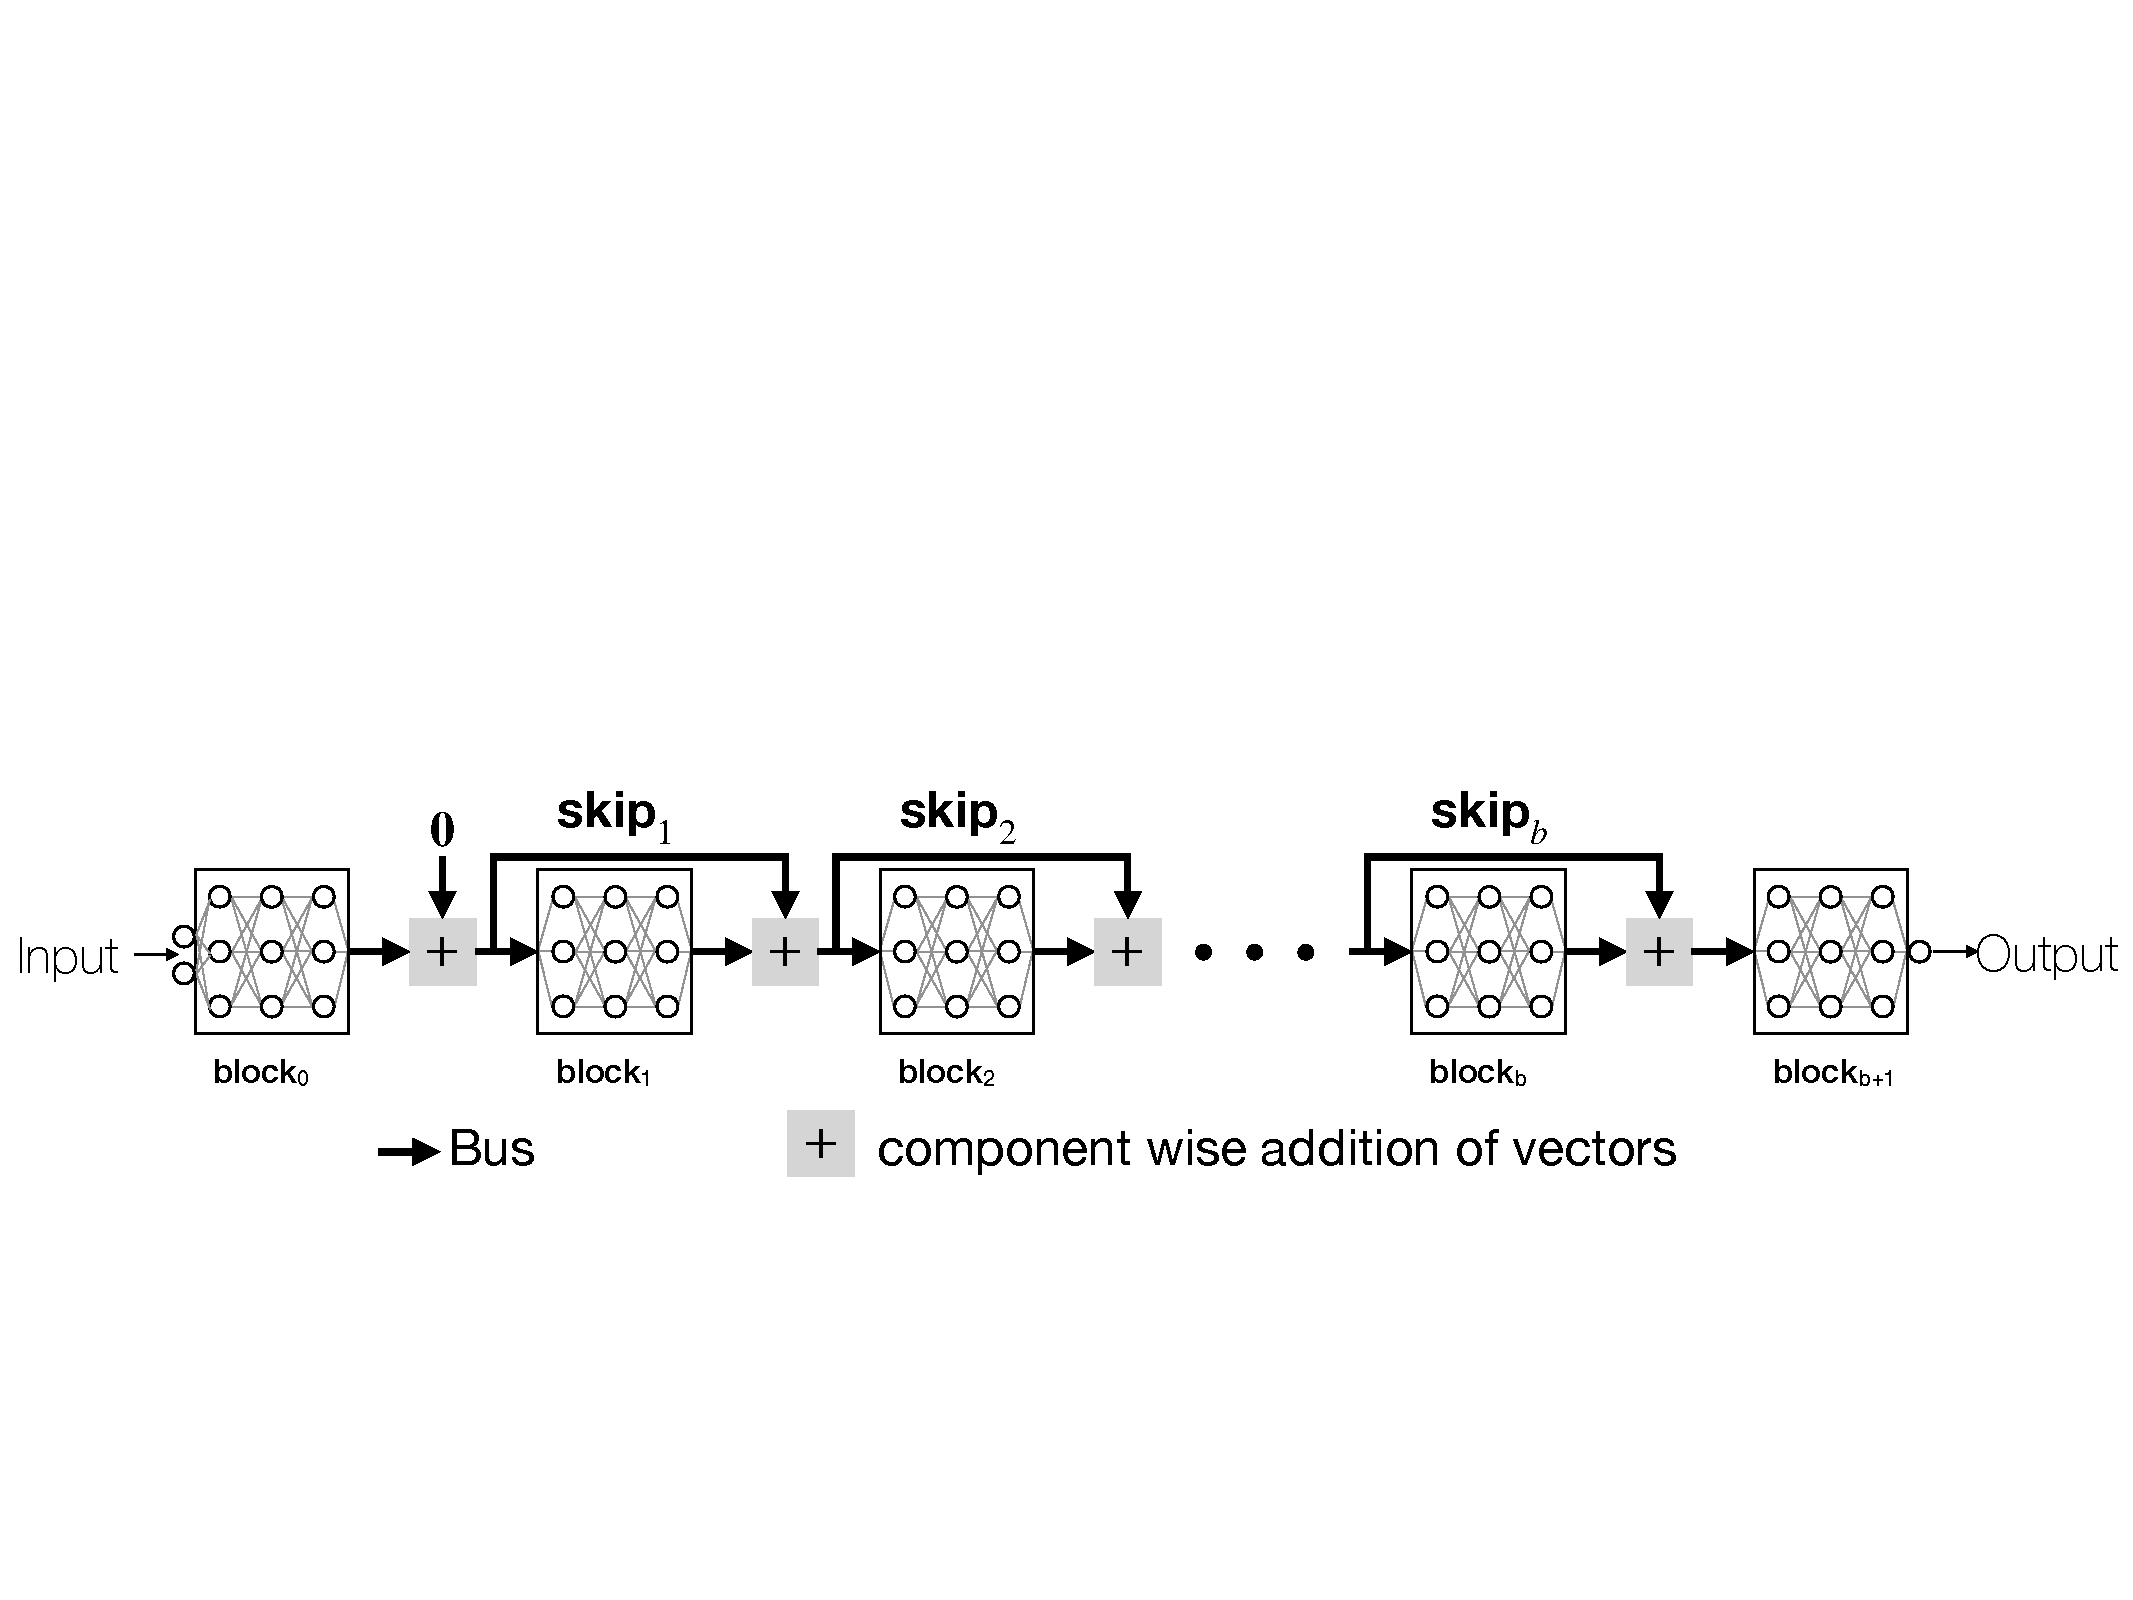
\includegraphics[scale=0.5]{figs/resnet.pdf}
}
\end{minipage}
\begin{minipage}{0.5\columnwidth}
\resizebox{\columnwidth}{!}{
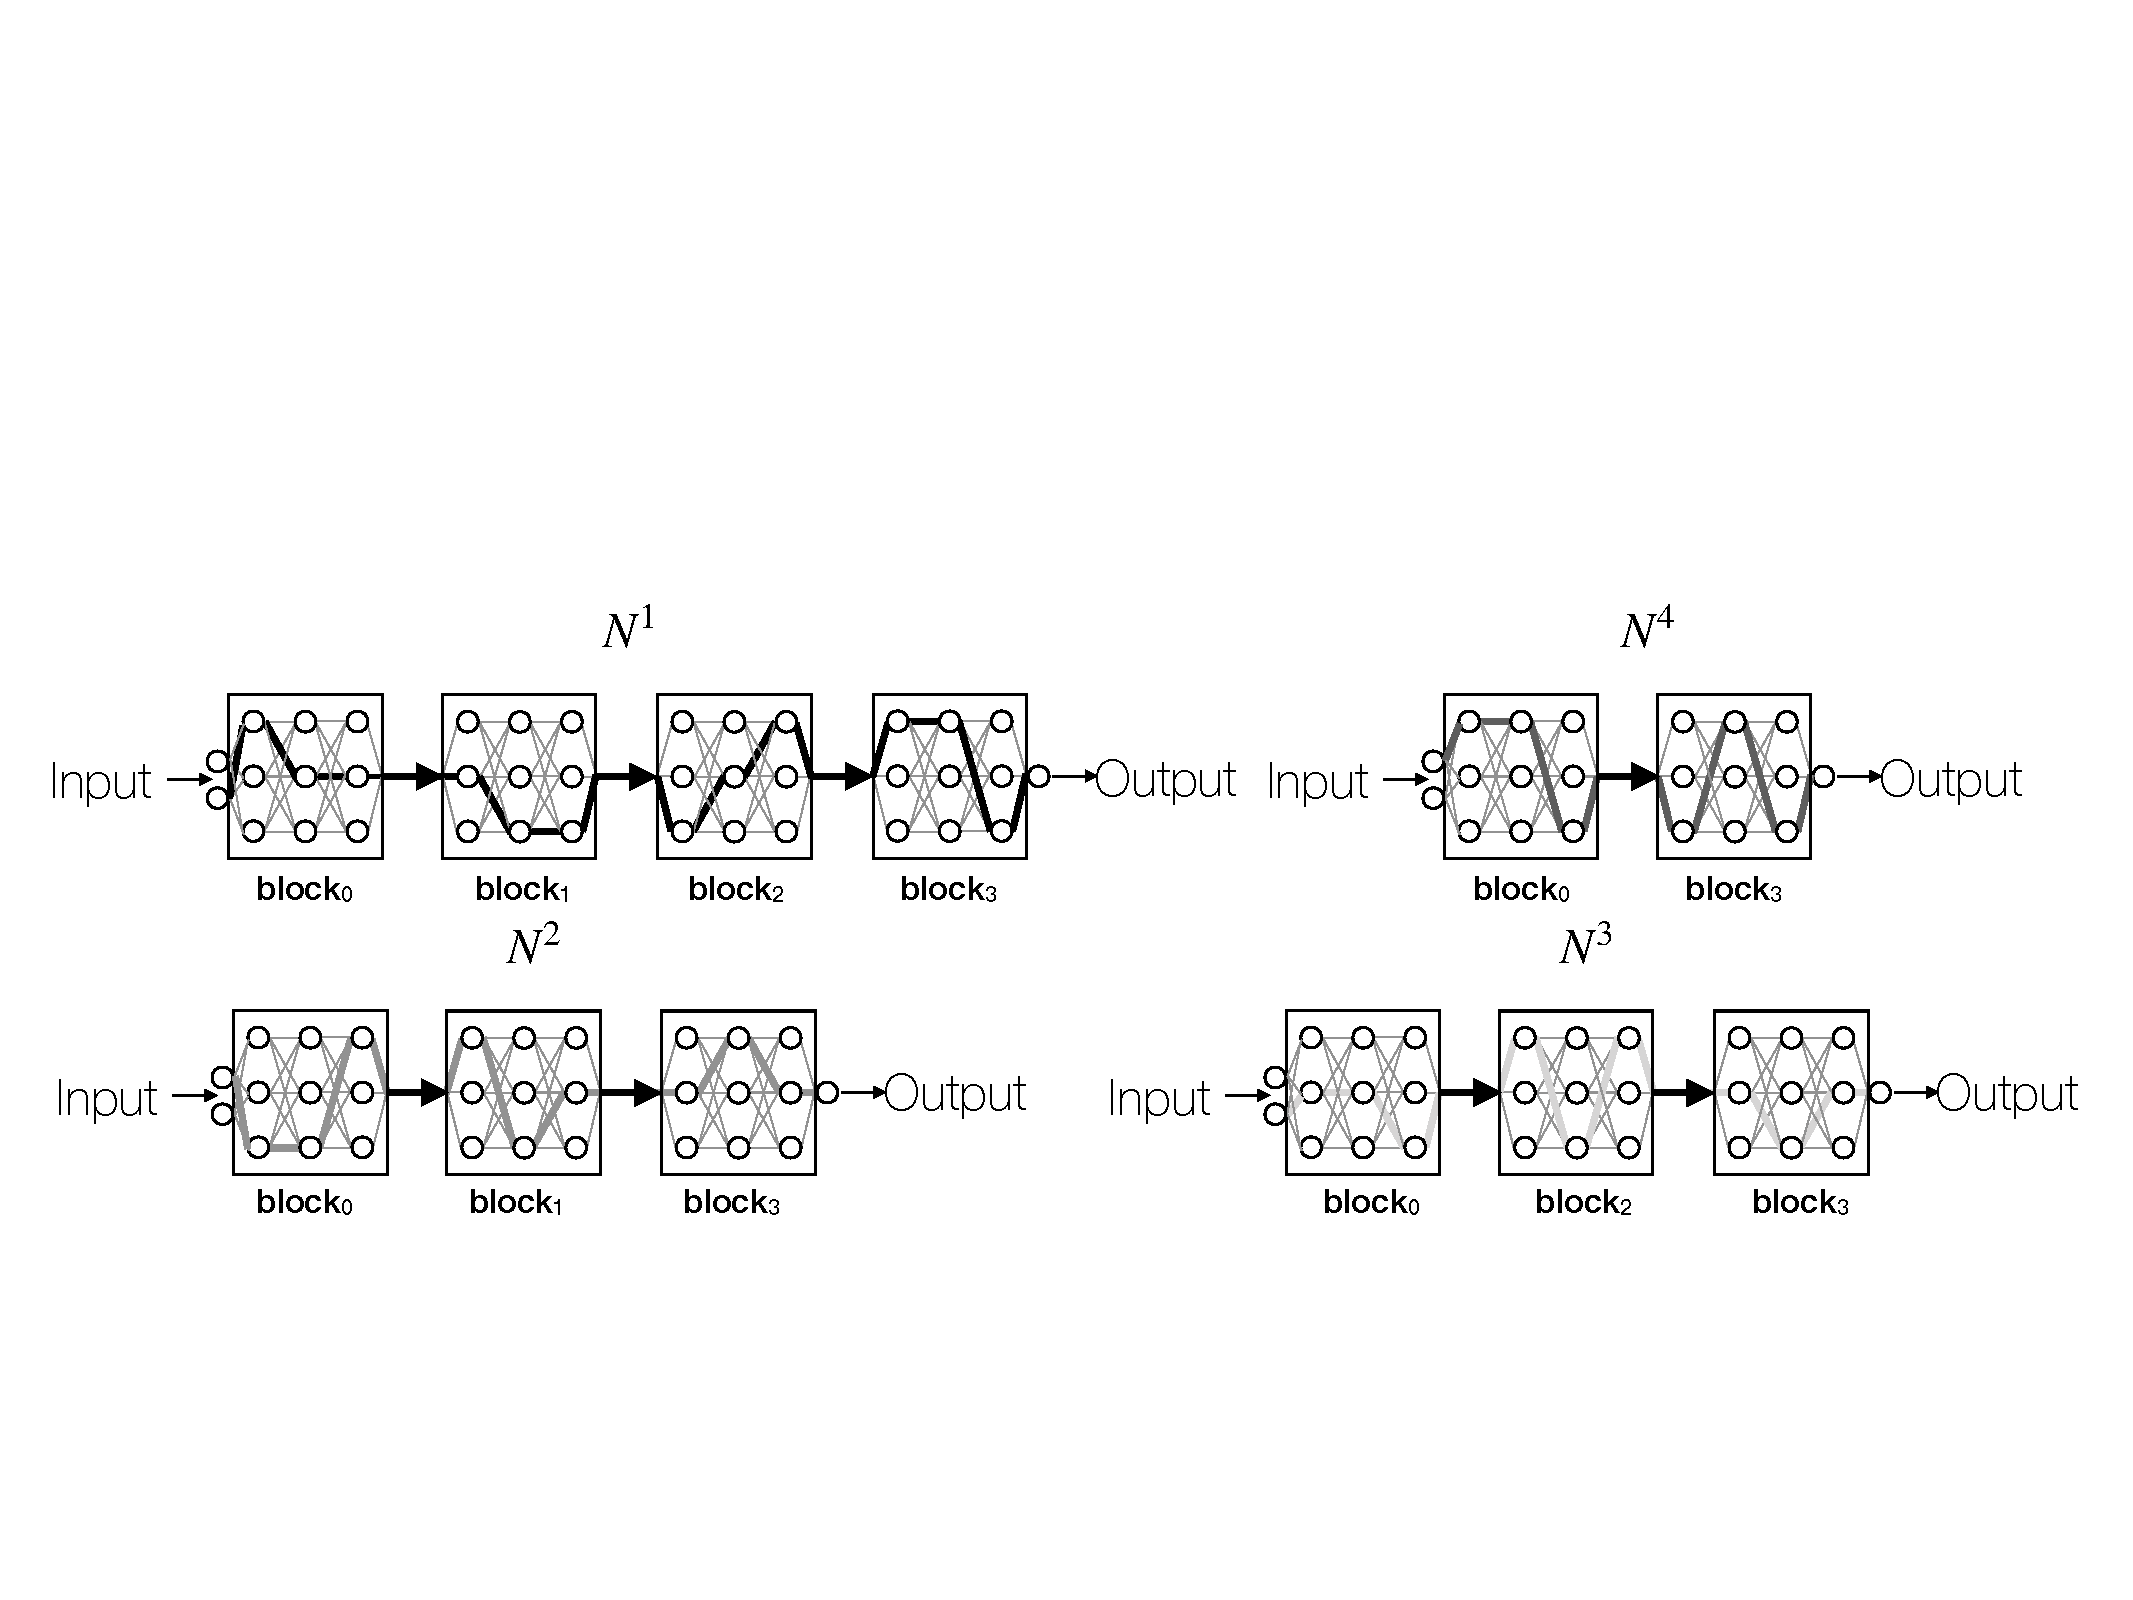
\includegraphics[scale=0.5]{figs/blocks.pdf}
}
\end{minipage}
\caption{\small{Figure on the left is the ResNet with $b$ skip connections and $(b+2)$ blocks. Figure on the right shows for $b=2$, the sub-FCNs $N^1$ obtained by skipping no blocks, $N^2$ and $N^4$ obtained by skipping block $1$ and $2$ respectively, and $N^3$ obtained by skipping both blocks $1$ and $2$.}}
\label{fig:resnet}
\end{figure}
\end{comment}
\begin{definition}\label{def:subfcdnn}[Sub FCNs]
Let $2^{[b]}$ denote the power set of $[b]$ and let $\J\in 2^{[b]}$ denote any subset of $[b]$. Define the`$\J^{th}$' sub-FCN of the ResNet to be the fully connected network obtained by (i) including  $\text{block}_{j},\forall j\in \J$  and (ii) ignoring $\text{block}_{j},\forall j\notin \J$. %(see \Cref{fig:resnet}).
\end{definition}
\begin{theorem}\label{th:res} 
Let $\text{NPK}^{\texttt{FC}}_{\J}$ be the NPK of the $\J^{th}$ sub-FCN, and $\bfc^{\J}$ (see Appendix for expansion of $\bfc^{\J}$) be the associated constant. Under \Cref{assmp:main}, we have:
\begin{align*}
\text{NTK}^{\texttt{RES}}\rightarrow \sum_{\J\in 2^{[b]}}  \bfc^{\J} \text{NPK}^{\texttt{FC}}_{\J}, \,\, \text{as}\,\,  w\rightarrow\infty
\end{align*}
\end{theorem}
%\textbf{Note.} The sub-FC-DNNs we refer to in \Cref{th:mainres} belong to (or are parts of) the feature network from which the gates are obtained. 
$\bullet$ \textbf{Ensemble.} To the best of our knowledge, this is the first theoretical result to show that ResNets have an ensemble structure, where  each kernel in the ensemble, i.e., $\text{NPK}^{\texttt{FC}}_{\J}$ corresponds to one of the $2^b$ sub-architectures (see \Cref{def:subfcdnn}). The ensemble behaviour of ResNet and  presence of $2^b$ architectures was observed by \cite{veit2016residual}, however without any concrete theoretical formalism. 

$\bullet$ The effect of \textbf{constant $\mathbf{1}$ input} is as before for kernels $\text{NPK}^{\texttt{FC}}_{\J}$ (if they are fully connected/convolutional networks with global average pooling) and holds for the overall kernel $\text{NTK}^{\texttt{RES}}$.

$\bullet$ \textbf{Destroying structure} \cite{veit2016residual} showed empirically that ``removing single layers from residual networks at test time does not noticeably affect their performance", and yet ``removing a layer from architecture such as VGG leads to a dramatic loss in performance". \Cref{th:res} can be seen to provide a theoretical justification for this empirical result. In other words, due to the ensemble structure a ResNet is capable of dealing with failure of components. While failure of component itself does not occur unless one makes them fail purposefully as done in \citep{veit2016residual},  the insight is that even if one or many of the kernels in the ensemble are corrupt and the good ones can compensate.% for them. 
%The main novelty in our paper compared to \citep{veit2016residual} is that we provide a mathematical framework and also the expression for the ensemble kernel. Thus, our results are theoretical and \citep{veit2016residual} presents empirical results without rigorous theory.

%In order to completely address the `black box'-ness issue, an ideal goal is to aim for theoretical results (supported by empirical evidence) on finite time learning in finite width \texttt{DGN-NO-ACT}. We find this goal is too hard at this stage and do not pursue the same. The next level is to analyse  the primal linearity and the dual linearity separately. Understanding the primal linearity has two parts to it (i) `what do the learnt pre-activations mean?', and (ii) `how are useful pre-activations learnt?'. The `what' question is \emph{post-hoc}, i.e., we can inspect the learnt pre-activations after training. However, we believe that in order to obtain domain specific insights on what the learnt pre-activations mean, we might require domain specific tools. For instance, in the case of `image classification', the pre-activations are the result of series of convolutions by `filter banks', and in order to do full justice, any visual interpretation should also tally with the results from `filter bank' theory. We defer the `what' question for future work. We also believe new theory is required to answer `how are useful pre-activations learnt?', and defer the same to future work. In this paper,  


%$\bullet$ We empirically show that \texttt{DGN-NO-ACT} performs comparably well on standard datasets. 

%$\bullet$ We restate the prior result for the fully connected case so as to explicitise the role of gates, depth and width. We extend the dual view theory to cover  convolutions with global pooling and skip connections.  We show empirically that the value network learns path-by-path and not layer-by-layer.




%A \texttt{DGN-NO-ACT} learns the relation $\hat{y}(x)=\ip{\phi_\Tf(x),v_{\Tv}}$, by learning simultaneously the feature and value network parameters. The pre-activations generated by the feature network trigger the gates thereby directly dictating the neural path feature $\phi_\Tf(x)$. It was shown that neural path features (i.e., the gates) are learnt during training and such learning improves generalisation \cite{npk}. Thus, while the learning in feature network is key, we reserve its theoretical study for future work. In this section, we will analyse the dual linearity, wherein, the theoretical results are in the \emph{inifinite width regime} which yield us a \emph{kernel} interperation, using which we probe into the properties of finite width networks. In other words, our aim is not to propose pure kernel methods with the kernel derived from an inifnite width DNN. 

%For the purpose of analysing the dual, we first explicitise in \Cref{th:fc} an unnoticed invariance property in the prior result of \cite{npk} for fully connected networks. In \Cref{th:conv,th:res} we also extend the dual formulation to cover the cases of convolutions with global pooling and skip connections. These results justify the constant $\mathbf{1}$ input to the value network of the \texttt{DGN-NO-ACT}. We also experimentally verify the constant $\mathbf{1}$ input as well as destroying the layer-by-layer structure of the gates does not degrade the performance. While these results are surprising and counter intuitive with respect to the primal view, they are follow in a straightforward manner from the results in the dual view, thereby underscoring the fact the value network indeeed computes path-by-path, and eliminating the `mystery' as to whether sophisticated structures are learnt layer-by-layer.

